\documentclass{article}

% if you need to pass options to natbib, use, e.g.:
%     \PassOptionsToPackage{numbers, compress}{natbib}
% before loading neurips_2024


% ready for submission
\usepackage{hyperref}       % hyperlinks
\usepackage[final]{neurips_2024}


% to compile a preprint version, e.g., for submission to arXiv, add add the
% [preprint] option:
%     \usepackage[preprint]{neurips_2024}


% to compile a camera-ready version, add the [final] option, e.g.:
%     \usepackage[final]{neurips_2024}


% to avoid loading the natbib package, add option nonatbib:
%    \usepackage[nonatbib]{neurips_2024}
\usepackage{graphicx}
\usepackage{natbib}
\usepackage{amsmath}
\usepackage[utf8]{inputenc} % allow utf-8 input
\usepackage[T1]{fontenc}    % use 8-bit T1 fonts
\usepackage{hyperref}       % hyperlinks
\usepackage{url}            % simple URL typesetting
\usepackage{booktabs}       % professional-quality tables
\usepackage{amsfonts}       % blackboard math symbols
\usepackage{nicefrac}       % compact symbols for 1/2, etc.
\usepackage{microtype}      % microtypography
\usepackage{xcolor}         % colors
\usepackage{bbm}
\usepackage{subcaption}

\graphicspath{/home/slaing/ML/2nd_year/sem2/research/uncertainty_report/figures/}

\title{Do Soft Labels Enhance Neural Network Training? \\ A Study on the CIFAR-10 Soft Dataset}


% The \author macro works with any number of authors. There are two commands
% used to separate the names and addresses of multiple authors: \And and \AND.
%
% Using \And between authors leaves it to LaTeX to determine where to break the
% lines. Using \AND forces a line break at that point. So, if LaTeX puts 3 of 4
% authors names on the first line, and the last on the second line, try using
% \AND instead of \And before the third author name.


\author{
	Sam Laing \\
	University of Tuebingen\\
	\texttt{sam.laing@student.uni-tuebingen.de}
}


\begin{document}

\maketitle


\begin{abstract}
	We explore the impact of training variants of ResNet architectures on CIFAR10 when soft labels are availible.  \\
	In particular, we implement Spectral Normalized Gaussian Processes (SNGP) and Deterministic Uncertainty Quantification and Monte Carlo Dropout on top of a small ResNet model. We then compare the robustness of models trained using the hard and soft CIFAR10 datasets.
	Furthermore, we investigate whether regularization techniques such as MixUp and CutMix can emulate the benefits using soft labels when training such networks . \\
	Our results show that no single model variant consistently excels across all metrics considered. However, soft labels generally enhance robustness, with the exception of calibration, which sees reduced performance. Furthermore, regularization techniques like MixUp and CutMix prove generally ineffective in replicating the benefits of soft labels.
\end{abstract}
\section{Introduction}
Image datasets with soft labels are often availible for free if multiple annotators are used in the labelling process. They can be thought of as a means of encoding some aleatoric uncertainty since if annotators disagree on a label image, it is likely that some cues are present in the image which are indicative of more than one of the possible classes. 

Typically, the label most frequently selected by annotators is chosen as the class label for each image. The soft label distribution is thus discarded in favour of a hard label dataset. We argue that this eliminates some rich information which could be learned by our model. Here we investigate the benefit of incorporating soft labels into the training process. 

Previous research (\cite{peterson2019humanuncertaintymakesclassification}) has shown that convolutional networks trained on CIFAR10 with soft labels have better robustness and marginally higher accuracy than their hard-labelled counterparts. 

We aim to systematically evaluate the impact of training neural networks on soft versus hard-labeled versions of the CIFAR-10 dataset. We compare the performance of uncertainty-estimating extensions on ResNet, across a range of metrics including accuracy, ECE, FGSM robustness and OOD detection. We also explore the possibility of using such techniques as Cutmix and Mixup to emulate the properties of a soft labelled dataset as well as the role of regularization techniques such as Monte Carlo Dropout and data augmentation. Our results provide insights into the trade-offs between these approaches and the potential benefits of leveraging soft labels for improved model robustness.
\section{Methods}
In this section we briefly introduce the different methods we applied along with the metrics used to benchmark each method. 
\subsection{ResNet Modifications Used}
\subsubsection*{Spectral Normalized Gaussian Process (SNGP)} 
As introduced by \cite{liu2020simpleprincipleduncertaintyestimation}, this method approximates a Gaussian process over the classifier’s output, yielding a principled measure of confidence in each prediction. By doing so, it provides uncertainty estimates that are particularly useful when the model encounters out-of-distribution data.

Additionally, SNGP applies spectral normalization between layers, which constrains the model’s Lipschitz constant to ensure that small input changes lead to proportionally small changes in the output. This Lipschitz constraint supports "distance awareness," meaning the model can better discern when inputs are near or far from the training distribution, further enhancing its robustness to unfamiliar data.

\subsubsection*{Deterministic Uncertainty Quantification (DUQ)}  
Introduced by \cite{duq} this technique uses a deep neural network as a feature extractor into an embedding space. It then learns a vector in the embedding space for each class which is referred to as a centroid. The centroids are updated continuously during training. 

A kernel function (in most cases RBF) is then used to to compute the distance of each feature output to each centroid. The predicted class is then chosen based on the closest centroid. The uncertainty is then determined by the exponentiated distance of the feature vector to the closest centroid. 
\\
A two sided gradient penalty was chosen as this was recommended by the authors. 

\subsubsection*{Monte Carlo Dropout} 
Dropout (\cite{JMLR:v15:srivastava14a}) is widely used in deep learning, initially introduced as a regularization technique. However, it can also be interpreted as a Bayesian approximation of a corresponding Gaussian process, as demonstrated by \cite{pmlr-v48-gal16}. When dropout is applied at inference time, it effectively functions as an on-the-fly ensembling method.

We therefore explore incorporating dropout into basic ResNet architectures. Given its regularization properties, we examine the effectiveness of dropout as an alternative to data augmentation, as well as the combined use of both techniques for enhanced model performance.
\subsubsection*{Mixup and CutMix}
Mixup was introduced by \cite{zhang2018mixupempiricalriskminimization} as a means of improving model generalization and adversarial robustness. The technique involves taking convex combinations of images and labels in the training phase, where the weight is drawn from a beta distribution centred at 0.5. 

CutMix was later designed by \cite{yun2019cutmixregularizationstrategytrain}. Effectively CutMix combines the ideas of Mixup and the regularization method Cutout (\cite{devries2017improvedregularizationconvolutionalneural}), which randomly masks out rectangular regions of each image in training. CutMix then cuts a rectangular region of one image and pastes it onto another image. The size and position of the rectangle is drawn from a Uniform distribution and the labels are then mixed with the ratio of the area of the cut-out image to the pasted image. 

We implement both these techniques. In an attempt to closely emulate the effect of soft label distribution, we only implement Mixup (resp. CutMix) on each iteration of the dataloader with some probability. The probability we ended up choosing was the entropy of the soft labelled distribution. 
\subsection{Metrics}
When it comes to test time, hard labels are used regardless of whether the model was trained with hard or soft labels. This is because hard labels are what we are actually interested in in production. 

We introduce the following notation for the metrics discussed below. \\
Let $h:\mathcal{X} \to \mathbb{R}^K$ denote the logit function of a trained classifier where $\mathcal{X}$ is the feature space and $K\in \mathbb{N}$ is the number of classes. \\
The classifier $f:\mathcal{X} \to \{1,\ldots,K\}$ is then defined by
\[
f(x) := \text{argmax}_{k\in\{1,\ldots,K\} }(\text{softmax}(h(x))_k)
\] 
Denote by $\mathcal{D}_{\text{test}} = \{(x_t, y_t)\}_{t=1} ^ {T} \subset \mathcal{X} \times \{1,\ldots,K\} $ the test set.  Where each $x_t\in\mathcal{X}$ is a test input and each $y_t\in\{1,\ldots,K\} $ is the corresponding ground truth label. 

We briefly discuss each metric used below.
\subsubsection*{Expected Calibration Error (ECE)} 
First introduced by \cite{guo2017calibrationmodernneuralnetworks}, the ECE is a typical metric recorded to indicate model calibration. \\
The ECE serves as an estimator for the following quantity:
\[
	E_{p\sim \hat{P}}\left[\mathbb{P}\left( \hat{Y} = Y | \hat{P} = p \right) - p \right]
\]
Where we denote by $\hat{Y}$ the predicted class and $\hat{p}$ the predicted confidence.\\
The approximation is computed by partitioning into M evenly spaced bins and taking the weighted averages of the confidences and accuracies within each bin. Explicitely, the ECE is given by:
\[
	\text{ECE} := \sum_{m=1}^{M} \frac{|B_m|}{T} \left| \text{acc}(B_m) - \text{conf}(B_m) \right|
\] 
Where
\[
\text{acc}(B_m) := \frac{1}{|B_m|} \sum_{i \in B_m} \mathbbm{1}_{y_i = \hat{y}_i} \quad , \quad 
\text{conf} = \frac{1}{|B_m|} \sum_{i \in B_m} \hat{p}_i
\]

We record the ECE of each model on the test set with $M=10$ 
\subsubsection*{Out of Distribution AUROC (OOD AUROC)} 
We also measure the OOD detection capabilities of each model we train, since it is a good indicator of model robustness. 
Since we invoke substantial data augmentation due to the small size of the CIFAR10 test set, we use SVHN data as our OOD data in favour of heavily augmented data from the same distribution. Each image in the SVHN dataset is of the same 32 $\times$ 32 $\times$ 3 size as in CIFAR10 and has different contents. It thus serves as excellent OOD data. 

We generate an OOD dataset of the same size as the test set. The ood datapoints are given label $0$ and the test (in distribution) set labels $1$. We then compute $\text{max}_k(h(x))$ for each $x\in\mathcal{D}_{\text{ood}} \cup \mathcal{D}_{\text{test}}$. The resulting AUROC on the binary classification problem is then recorded. \\
\subsubsection*{Fast Gradient Sign Method (FGSM) accuracy decrease}
Another metric considered was the decrease in accuracy after applying a FGSM attack (\cite{goodfellow2015explainingharnessingadversarialexamples}) to every correctly predicted test point. \\
Namely, one selects a perturbation size $\varepsilon \in \mathbb{R}_{>0}$ and then "attacks" the input image $x$ as follows
\[
x_{\text{adv}} = x + \varepsilon \text{sign}(\nabla_x L(x,y; \theta))
\] 
Where $L$ is the loss function of the network.

Since we apply normalization to the test images, one must first denormalize the image, exact the attack and then renormalize.  

A value of $\varepsilon =0.005$ was chosen as the perturbation size after some consideration. 

We view this metric as an indicator of the adversarial robustness of each model. 
\subsubsection*{Accuracy}
Of course the accuracy on the test set defined by $\text{acc}(f, \mathcal{D}_{\text{test}}) = \sum_{j=1}^{T} {\mathbbm{1}_{f(x_j) = y_j}}$ was also recorded.


\subsubsection*{A comment on proper scoring rules} 
We also considered the cross entropy loss and Brier score since they are proper scoring rules. 

Arguably this is an unfair comparison since we test on hard labels and our soft-labelled classifiers were trained to predict a distribution. 
\section{Experimental Outline}
\subsection{Comparison of Uncertainty Methods}
\subsubsection*{Network Architecture}
All experiments were conducted using a small ResNet model with 20 layers. This model consisted of around $270,000$ parameters. We note preliminary investigations indicated that increasing the network depth did not lead to improved model performance, nor was double descent observed, even when the depth was increased to 98 layers (resulting in a model with over $1.5$ million parameters). This can likely be attributed to the to the relatively small size of the training dataset.
\subsubsection*{Optimization}
We employed a Stochastic Gradient Descent (SGD) optimizer with Nesterov momentum as is standard practice. A learning rate warmup scheduler was initially applied, followed by a Multi-Step learning rate scheduling with frequent updates. This strategy was found to improve both training speed and final model accuracy. Models were trained for 230 epochs with early stopping employed to choose the model with the lowest validation loss. In practice, convergence usually occurred between 150 and 200 epochs but on occasion further training improved accuracy marginally. 
\\
We found the use of a warm up learning rate scheduler was very helpful for training DUQ and SNGP models and had minimal effect on vanilla ResNet and Dropout models.  
\subsubsection*{Data Splits}
The dataset was divided into training, validation, and test sets using an $80$-$5$-$15$ split. Specifically, $8,000$ images were allocated for training, $500$ for validation, and $1,500$ for testing.
\subsubsection*{Data Augmentation}
For models trained on this smaller dataset, data augmentation proved essential, particularly for the model variations in which dropout couldn't be applied. Without augmentation, the models suffered from overfitting and degraded performance, usually around 15\% lower accuracy was observed.

In particular, through extensive experimentation, we found that the use of ColorJitter, RandomHorizontalFlip, RandomRotation(10) and  RandomResizedCrop (in this order) resulted in the models of highest accuracy without significantly deteriorating other model characteristics. 
\subsubsection*{Loss Functions}
For all models except DUQ, the standard Cross-Entropy loss function was used. 
For an individual data point $(x,y) \in \mathcal{X} \times \mathcal{Y}$, the model predicts a vector $p_{\theta}(x) := \text{softmax}(h(x)) \in\Delta^{K-1}$ representing a categorical distribution in the label space. The cross entropy loss against the ground truth label $y\in \Delta^{K-1}$ is then given by:
\[
	L(p_{\theta}(x), y) = -\sum_{k=1}^{K} {y_k \log (p_{\theta}(x)_k)}
\]
We note that in the case of soft labels, each $y_k$ can generally assume values outside of $\{0,1\} $. Therefore the loss function cosists of more than one component. This is in contrast to the hard labelled case where only one component of $y$ is non-zero.

For the DUQ models, we employed the same loss function introduced in \cite{duq}. Namely if we consider $g_{\theta}: \mathcal{X} \to \mathbb{R}^{F}$ as the embedding portion of the network and $\kappa: \mathbb{R}^{F} \times \mathbb{R}^F\to \mathbb{R}_{\ge_0}$ the exponentiated distance function, the loss function is then given by:
\[
L(x,y) = -\sum_{k=1}^{K} {y_k}\log \kappa(g_{\theta}, e_k) + (1-y_k) \log(1-\kappa(g_{\theta}, e_k))
\] 
where $e_k$ is the  $k^{\text{th}}$ centroid learned by the DUQ network.
\subsubsection*{Models Trained}
We used several different model configurations: SNGP, DUQ, a basic model without dropout or data augmentation, a basic model with dropout but no data augmentation and a basic model with data augmentation but no dropout. For each configuration, we trained the following variations: one with soft labels, one with hard labels and one with hard labels, one with hard labels with Mixup applied and one with hard labels with CutMix applied.

In addition, we applied MixUp and CutMix to the soft-labeled dataset to investigate whether these techniques could further enhance performance when combined with soft labels. This approach was chosen both to assess potential gains in robustness and calibration and to ensure a comprehensive analysis, distinguishing the effects of hard versus soft labels from those attributable to MixUp and CutMix themselves.

The probability value chosen for the Mixup and CutMix methods was chosen as the entropy of the train dataset with soft labels. The idea behind this was to create a simlar degree of "softness of labels" with the hard dataset.

In total, we trained $30$ distinct model types. For fairness and reproducibility, each model was trained using five different random seeds. The random seed determined the initialization, the torch (\cite{NEURIPS2019_9015}) mini-batching and training and the train-test dataset splits. The recorded metrics were averaged across these runs, allowing for the computation of standard error. This then allows for stronger statistical comparisons between performances.
\section{Results}
The performance metrics of each model is listed in \autoref{tab:model_comparison}


\begin{table}[ht]
\caption{Comparison of different models.\\
For each of the 5 model types, we put the best metric in bold. The best metric across all models is highlighted in red.}
\centering
\resizebox{\textwidth}{!}{%
\begin{tabular}{lcccc}
\toprule
Model Type & Accuracy & OOD AUROC & ECE & Attack Decrease \\
\midrule
basic, soft labels  & 82.917 $\pm$ 0.841 & 0.775 $\pm$ 0.0427 & 0.0905 $\pm$ 0.0029 & \textbf{0.3518 $\pm$ 0.0152} \\
basic, hard labels  & 81.367 $\pm$ 0.601 & 0.711 $\pm$ 0.0540 & \textbf{\textcolor{red}{0.0463 $\pm$ 0.0028}} & 0.4412 $\pm$ 0.0181 \\
basic, soft labels,  Mixup  & 82.150 $\pm$ 1.415 & \textbf{0.785 $\pm$ 0.0545} & 0.103 $\pm$ 0.0068 & 0.3562 $\pm$ 0.0173 \\
basic, hard labels,  Mixup  & 81.650 $\pm$ 0.580 & 0.682 $\pm$ 0.0757 & 0.0703 $\pm$ 0.0025 & 0.4448 $\pm$ 0.0137 \\
basic, soft labels,  CutMix & \textbf{\textcolor{red}{83.517 $\pm$ 1.398}} & 0.748 $\pm$ 0.0790 & 0.108 $\pm$ 0.0033 & 0.3885 $\pm$ 0.0097 \\
basic, hard labels,  CutMix & 82.683 $\pm$ 0.500 & 0.527 $\pm$ 0.0669 & 0.0824 $\pm$ 0.0028 & 0.4645 $\pm$ 0.0214 \\
\midrule
basic, soft labels, dropout, no aug  & 78.187 $\pm$ 0.662 & 0.658 $\pm$ 0.0673 & 0.111 $\pm$ 0.0036 & \textbf{0.1753 $\pm$ 0.0084} \\
basic, hard labels, dropout, no aug ,  & 77.653 $\pm$ 0.959 & 0.588 $\pm$ 0.0813 & \textbf{0.0569 $\pm$ 0.0022} & 0.2028 $\pm$ 0.0080 \\
basic, soft labels, dropout, no aug Mixup,  & 78.787 $\pm$ 0.691 & \textbf{0.689 $\pm$ 0.0633} & 0.126 $\pm$ 0.0030 & 0.1763 $\pm$ 0.0128 \\
basic, hard labels, dropout, no aug Mixup,  & 78.147 $\pm$ 0.875 & 0.532 $\pm$ 0.0992 & 0.0880 $\pm$ 0.0028 & 0.1927 $\pm$ 0.0093 \\
basic, soft labels, dropout, no aug , CutMix & \textbf{80.147 $\pm$ 0.662} & 0.659 $\pm$ 0.0754 & 0.132 $\pm$ 0.0065 & 0.1774 $\pm$ 0.0060 \\
basic, hard labels, dropout, no aug , CutMix & 78.560 $\pm$ 0.719 & 0.443 $\pm$ 0.0861 & 0.0948 $\pm$ 0.0029 & 0.1950 $\pm$ 0.0073 \\
\midrule
basic, soft labels, dropout  & 82.933 $\pm$ 0.144 & \textbf{0.785 $\pm$ 0.0365} & 0.0999 $\pm$ 0.0008 & 0.1518 $\pm$ 0.0037 \\
basic, hard labels, dropout  & 82.400 $\pm$ 0.536 & 0.548 $\pm$ 0.0257 & \textbf{0.0702 $\pm$ 0.0009} & 0.1687 $\pm$ 0.0005 \\
basic, soft labels, dropout, Mixup  & 82.444 $\pm$ 0.851 & 0.734 $\pm$ 0.0180 & 0.110 $\pm$ 0.0035 & \textbf{\textcolor{red}{0.1407 $\pm$ 0.0059}} \\
basic, hard labels, dropout, Mixup  & 82.178 $\pm$ 0.362 & 0.636 $\pm$ 0.0393 & 0.0882 $\pm$ 0.0042 & 0.1751 $\pm$ 0.0079 \\
basic, soft labels, dropout CutMix & \textbf{83.378 $\pm$ 0.939} & 0.761 $\pm$ 0.0381 & 0.117 $\pm$ 0.0012 & 0.1578 $\pm$ 0.0047 \\
basic, hard labels, dropout, CutMix & 82.711 $\pm$ 1.050 & 0.558 $\pm$ 0.0268 & 0.0940 $\pm$ 0.0016 & 0.1731 $\pm$ 0.0079 \\
\midrule
duq, soft labels & 81.907 $\pm$ 1.203 & \textbf{0.797 $\pm$ 0.0755} & 0.693 $\pm$ 0.0106 & 0.4217 $\pm$ 0.0208 \\
duq, hard labels & 81.653 $\pm$ 1.025 & 0.667 $\pm$ 0.0738 & 0.6917 $\pm$ 0.0078 & 0.4269 $\pm$ 0.0270 \\
duq, soft labels, Mixup & \textbf{82.000 $\pm$ 1.077} & 0.714 $\pm$ 0.0199 & 0.694 $\pm$ 0.0090 & \textbf{0.4097 $\pm$ 0.0144} \\
duq, hard labels, Mixup & 80.907 $\pm$ 1.216 & 0.604 $\pm$ 0.0339 & \textbf{0.685 $\pm$ 0.0097} & 0.4099 $\pm$ 0.0184 \\
duq, soft labels, CutMix & 81.920 $\pm$ 1.573 & 0.717 $\pm$ 0.0289 & 0.692 $\pm$ 0.0135 & 0.4343 $\pm$ 0.0172 \\
duq, hard labels, CutMix & 81.587 $\pm$ 1.670 & 0.617 $\pm$ 0.0781 & 0.690 $\pm$ 0.0146 & 0.4299 $\pm$ 0.0194 \\
\midrule
sngp, soft labels  & 80.800 $\pm$ 1.180 & \textbf{\textcolor{red}{0.844 $\pm$ 0.0316}} & 0.0892 $\pm$ 0.0042 & \textbf{0.3555 $\pm$ 0.0084} \\
sngp, hard labels  & 80.667 $\pm$ 1.304 & 0.779 $\pm$ 0.0578 & \textbf{0.0472 $\pm$ 0.0026} & 0.4425 $\pm$ 0.0128 \\
sngp, soft labels,  Mixup  & \textbf{81.080 $\pm$ 0.795} & 0.743 $\pm$ 0.0685 & 0.1032 $\pm$ 0.0045 & 0.3623 $\pm$ 0.0124 \\
sngp, hard labels,  Mixup  & 80.893 $\pm$ 0.599 & 0.670 $\pm$ 0.0706 & 0.0689 $\pm$ 0.0029 & 0.4548 $\pm$ 0.0129 \\
sngp, soft labels, CutMix & 80.947 $\pm$ 0.932 & 0.752 $\pm$ 0.0634 & 0.1030 $\pm$ 0.0015 & 0.3821 $\pm$ 0.0130 \\
sngp, hard labels CutMix & 80.853 $\pm$ 0.698 & 0.592 $\pm$ 0.0620 & 0.0726 $\pm$ 0.0028 & 0.4624 $\pm$ 0.0187 \\
\bottomrule
\end{tabular}%
}
\label{tab:model_comparison}
\end{table}
\subsubsection*{Soft labels improve accuracy - but not by much}
We remark that due to only having access to $8,000$ training points, it was difficult to acheive a model accuracy in excess of 85\%. This is in line with \cite{peterson2019humanuncertaintymakesclassification} where it was also the case.  

While there is no great discrepency in accuracy between models, we observe that generally the use of soft labels slightly improves the accuracy of each model. Moreover, usually the use of Mixup and CutMix slightly improved model accuracy though not to any significant degree. 

We observe that the dropout models without data augmentation struggled to keep up with all other models accuracy-wise and generally suffered worse performance. When we tried any other model (vanilla ResNet, DUQ and SNGP) without augmentation, performance was substantially worse even when the weight decay term was substantially increased in the optimizer.  
\subsubsection*{Mixup and CutMix deteriorate OOD detection for hard labels}
When it comes to the OOD performance of each model, we again observe that every model trained with soft labels outperformed it's hard counterpart. Sometimes the discrepency in OOD detection capabilities was very large whereas other times not as substantial. 

We observe that the SNGP models generally produced the best OOD detectors although only the dropout model with no data augmentation showed very poor OOD detection performance. 

The use of Mixup and CutMix almost always decreased the OOD detection capabilities of hard-labelled models significantly and did not do so to nearly the same extent for the soft-labelled counterparts.
\subsubsection*{Soft labels make the ECE worse}
We make two key observations here.

Firstly, the DUQ model resulted in extremely high ECE values, in most cases almost an order of magnitude larger than the other models. Upon investigation, we found that the DUQ models seemed to produce softmax outputs with extremely high entropy relative to the other models. Generally the softmax outputs were not confident in their predictions. Although the accuracy of the DUQ models was no worse than other models. 

It appears as though this is an effect of overparametrization. Indeed, applying DUQ produces a model with more than three times the number of parameters as the vanilla ResNet. In contrast applying SNGP only only increases the total number of parameters by around 20\%. Explicitely, the vanilla ResNet model has $272,474$ parameters, the SNGP model had $349,284$ parameters and the DUQ model had $927,834$ parameters. 

Secondly, we observe that the ECE of the models trained on soft labels was always higher than the same model when trained on hard labels. Models trained on soft labels are trying to learn a more complex categorical distribution for each image. We considered the reliability diagrams of the basic ResNet models trained on hard and soft labels as we see in \autoref{fig:2x2grid}. We see that from the reliability diagrams alone, the models appear to have poor calibration. However upon inspection of the proportion diagrams (a histogram visualising the proportion of predictions falling into each bin), we see that both the hard and soft models predict with high confidence the majority of time and are usually correct in doing so. It is only on rare occurances that the models predict with confidences lower than 90\%. 
The models trained on soft labels are encouraged to predict with lower confidences more often. Therefore the ECE ends up being higher since the model has larger discrepency between confidence and true accuracy for lower confidence values. 

The reliability diagrams for the dropout and SNGP models looked quite similar. On the other hand, the DUQ model almost never predicted any class with confidence greater than 20\%. This was likely due to the overparametrization effect discussed above. \\
The use of Mixup and CutMix on hard labels always increased the ECE. From inspection of the relibility and proportion diagrams, we conclude that this is a similar phenomenon to the soft labels but to a somewhat lesser extent. 

\begin{figure}[ht]
    \centering
    \begin{minipage}{0.45\linewidth}
        \centering
        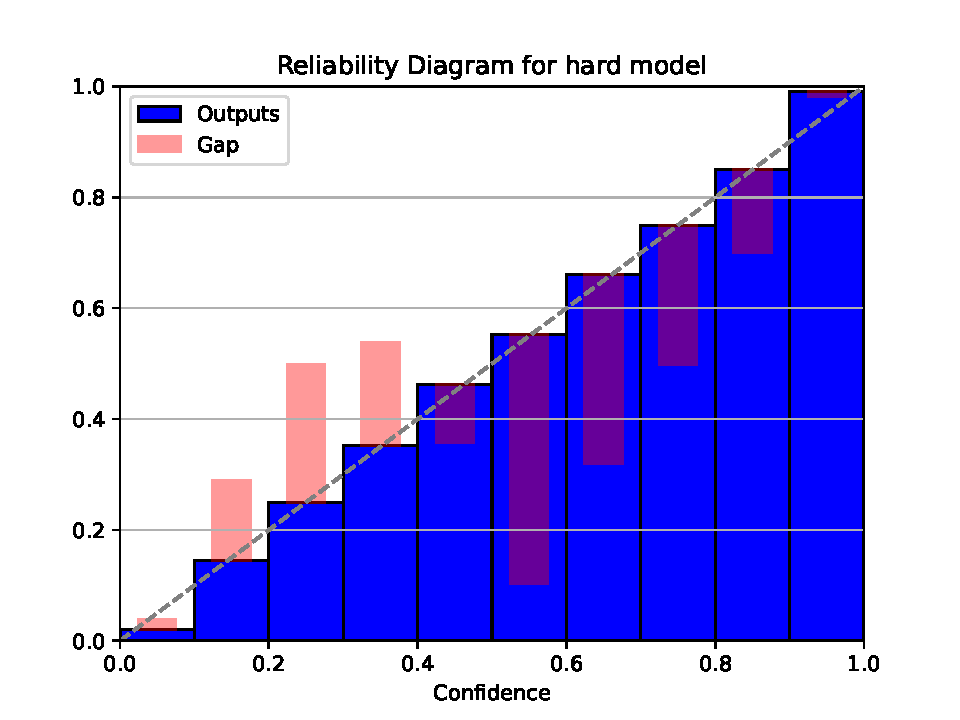
\includegraphics[width=\linewidth]{/home/slaing/ML/2nd_year/sem2/research/uncertainty_report/figures/hard_reliability_diagram.pdf}
    \end{minipage}
    \hfill
    \begin{minipage}{0.45\linewidth}
        \centering
        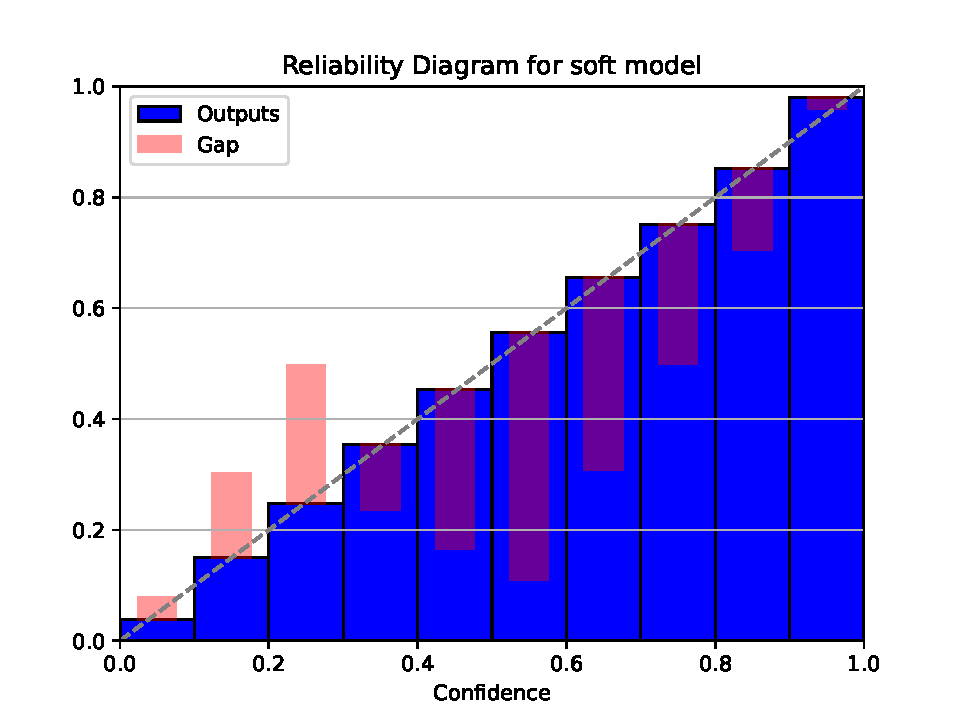
\includegraphics[width=\linewidth]{/home/slaing/ML/2nd_year/sem2/research/uncertainty_report/figures/soft_reliability_diagram.pdf}
    \end{minipage}
    \vfill
    \begin{minipage}{0.45\linewidth}
        \centering
        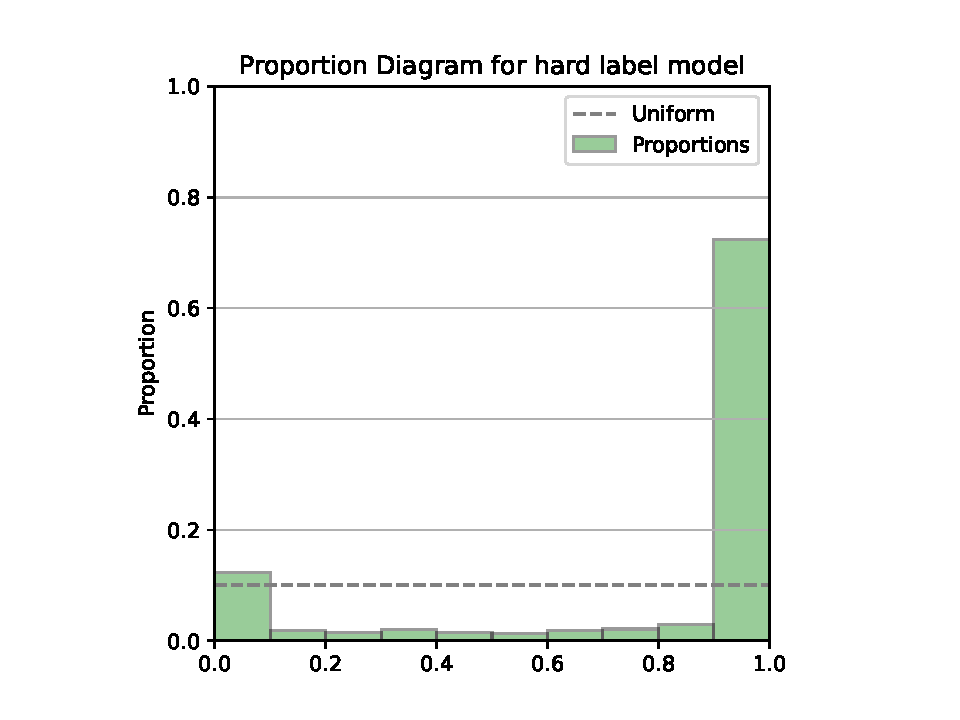
\includegraphics[width=\linewidth]{/home/slaing/ML/2nd_year/sem2/research/uncertainty_report/figures/hard_proportion_diagram.pdf}
    \end{minipage}
    \hfill
    \begin{minipage}{0.45\linewidth}
        \centering
        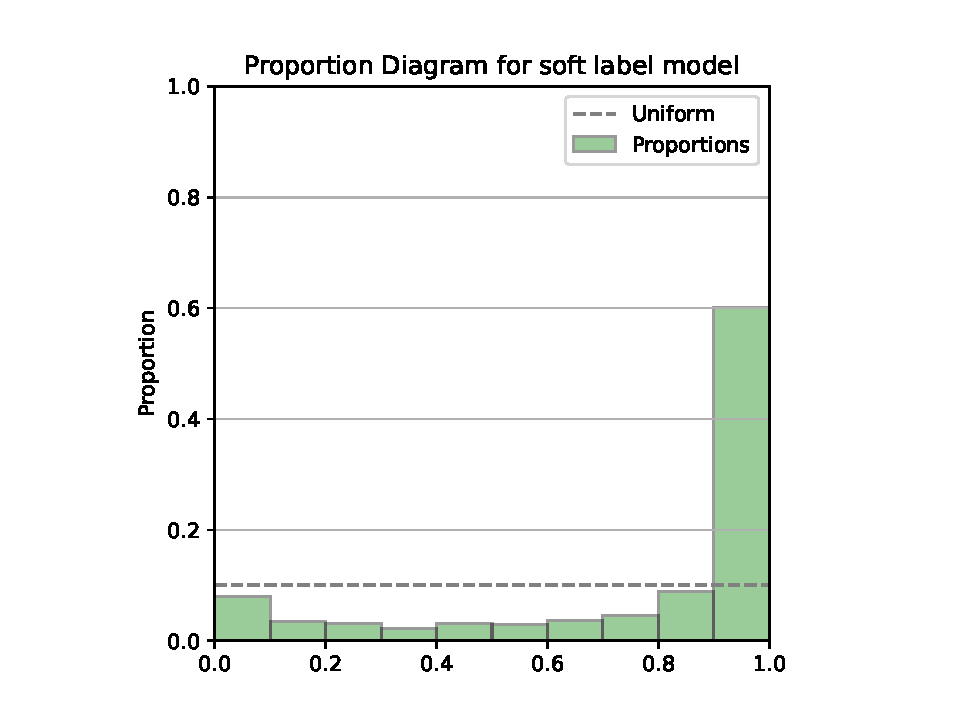
\includegraphics[width=\linewidth]{/home/slaing/ML/2nd_year/sem2/research/uncertainty_report/figures/soft_proportion_diagram.pdf}
    \end{minipage}
    \caption{Comparison of Hard and Soft Label Reliability and Proportion Diagrams}
    \label{fig:2x2grid}
\end{figure}


\subsubsection*{Dropout best adversarial defender }
The dropout models significantly outperformed all others with respect to adversarial robustness. The dropout technique we implemented involved ensembling at both train and test time. This ensembling-on-the-fly effect seemed to provide a significantly higher degree of adversarial robustness than any other methods applied. 

We also observe that again, models trained with soft labels always resulted in better adversarial robustness compared to the same models trained with hard labels. This was something already reported for basic ResNet architectures in \cite{peterson2019humanuncertaintymakesclassification} but we see that this holds true across all model types implemented. 
 
\subsubsection*{Log Loss and Brier Score}
So as not to overcrowd the table (\autoref{tab:model_comparison}) we don't include these results but we comment that the log loss score was comparable between the hard and soft label models with the hard label models with slightly lower values across all models. 

On the other hand, the Brier score was consistently and significantly lower for models trained with soft labels in comparison to the same models trained with hard labels. This was somewhat surprising since we evaluated the model trained with soft labels with hard labels. 
\section{Conclusion}
In this work, we explored the impact of training a ResNet model with soft labels using various techniques, including Mixup and CutMix, across multiple evaluation criteria: out-of-distribution (OOD) awareness, adversarial robustness, calibration, Brier Score, Log Loss and accuracy. Our investigation aimed to assess the benefits of having access to a soft labelled dataset and whether these data augmentation methods could replicate the benefits of training with soft labels.

Our findings indicate that Mixup and CutMix did not improve the robustness of models trained with hard labels to the same extent as those with soft labels. The distinct properties of the soft-label CIFAR10 dataset could not be effectively reproduced through these techniques. On the other hand, applying Mixup and CutMix to models trained on soft labels resulted in improved accuracy, albeit at the cost of decreased robustness, particularly in adversarial settings.

Among the methods examined, SNGP on soft labels demonstrated superior OOD detection performance, while Monte Carlo Dropout emerged as the most effective approach for adversarial robustness. This suggests that the optimal model choice depends on the specific robustness criterion, as no single approach consistently outperformed others across all metrics.

A key insight from our study is that access to soft labels during training generally improved model performance across most metrics, with the exception of calibration where the situation is more nuanced. This highlights the trade-offs when balancing accuracy and robustness in model selection, and suggests that having access to soft labels during training affords a number of upsides. 

\section{Potential Future Work}
While this research provided valuable insights into the impact of soft labels on model performance, several avenues remain open for further exploration.

Our findings revealed that Monte Carlo Dropout significantly enhanced adversarial robustness compared to other methods. It would be worthwhile to extend this investigation by exploring the effects of alternative ensembling techniques, which may offer similar or improved robustness.

Additionally, exploring different approaches to capturing uncertainty in model predictions could lead to further advancements. Methods such as Mahalanobis distance-based OOD detection (\cite{anthony2023usemahalanobisdistanceoutofdistribution}) and classifiers like HET-XL (\cite{collier2023massivelyscalingheteroscedasticclassifiers}
) and their integration with soft-label training warrants investigation.

Moreover, there are other approaches to try to emulate soft labels. One well known example is simply label smoothing but other interesting methods have been proposed such as Meta learning (\cite{vyas2020learningsoftlabelsmeta}) where soft labels are learned during the training process. It would be interesting to explore the interplay of such approaches with uncertainty aware networks. 
\appendix
% Bibliography Section
\bibliographystyle{plainnat} % Choose plainnat or abbrvnat, etc.
\bibliography{references}    % The name of your .bib file without the .bib extension


\end{document}
